\makeatletter
\def\input@path{{../../}}
\makeatother
\documentclass[../../main.tex]{subfiles}

\graphicspath{
	{../../img/}
	{../img/}
	{img/}
}

\begin{document}
	
\begin{proof}
	Для фиксированного $ z \in \C $ и $ R > 0 $ ?не понял, что тут? 
	в плоскости \encircle{t} окружность 
	\[ l_R = \{ t \in \C | \abs{t - z} = R\} \]. 
	Тогда из \eqref{lec32:7} при $ n = 1 $ имеем:
	\[
	f'(z) = \dfrac{1}{2\pi i} \oint\limits_{l_R} 
	\dfrac{f(t)}{(t - z)^2} dt \implies
	\abs{f'(z)} \leq \dfrac{1}{2\pi}
	\oint\limits_{l_R} \dfrac{\abs{f(t)}}{\abs{t - z}^2}
	\abs{dt} \leq
	\begin{bmatrix}
		\abs{f(t)} \leq M \\
		\abs{t - z} = R
	\end{bmatrix} \leq \dfrac{M}{2\pi R^2}
	\oint\limits_{l_R} \abs{dt} =
	\dfrac{M}{2\pi R^2}
	\]
	Длина $ l_r = \dfrac{M}{2\pi R^2} \cdot 2R = \dfrac{M}{R} $.
	Из полученного неравенства: $ \abs{f'(z)} \leq 
	\dfrac{M}{R} $ в силу того, что $ M = const $ не 
	зависит от $ R > 0 $ при $ R \to +\infty $ имеем:
	\[
	\abs{f'(z)} \leq 0 \implies 
	\abs{f'(z)} = 0 \implies 
	f'(z) = 0 \implies 
	f(z) = const \in \C
	\] в силу критерия ?пост.? ФКП.
\end{proof}
\begin{rem}
	Теорема Лицвилля показывает, что если ФКП $ f(z) \not\equiv const $,
	то в $ \C $ у неё возможно есть особенности, т.~к.
	она не может быть аналитической всюду в $ \C $.
\end{rem}
С другой стороны, целые ФКП $ \not\equiv const $ не могут быть ограничены в $ \C $.
Отсюда, в частности следует, что ???беск. дифф??? ФКП
является целыми и неограниченными в отличие от действительного 
случая $ \sin x $ и $ \cos x, x \in \R $, когда $ \abs{\sin x} \leq 1,\ 
\abs{\cos x} \leq 1,\ \forall x \in \R $. 
Здесь, не смотря на выполнение основного тригонометрического тождества 
из него не следует ограниченность комплексных тригонометрических функций $ 
\sin z,\cos z $. Например, если $ z = iy $, то
$ \cos z = \cos iy = \ch y
\underset{y \to \infty}{\to} \infty$.

\begin{crl}[основная теорема алгебры]
	Если многочлен $ P_n(z) = c_0 + c_1z + \dots + c_nz^n,\ c_k \in \C,
	k = \overline{0, n}, c_n \neq 0 $, имеет $ n \geq 1 $, то уравнение $ P_n(z) = 0 $ имеет хотя бы 1 комплексный корень.
\end{crl}
\begin{proof}
	Пусть $ P_n(z) \neq 0 \forall z \in \C $.
	Тогда $ f(z) = \dfrac{1}{P_n(z)} $ не имеет особенностей в $ \C $ 
	и будет дифференцируема $ \forall z \in \C,\
	f'(z) = -\dfrac{P_n'(z)}{P_n(z)} $. Значит, 
	$ f(z) $~--- целая ФКП.
	
	Учитывая, что $ f(\infty) = 0 \implies
	\exists R = const > 0:\quad \forall z \in \C \implies
	f(z) $~--- ограничена. Кроме того, по теореме Вейерштрасса, будет 
	ограничена и на компакте $ \abs{z} \leq R $.
	Значит, $ f(z) $ ограничена на $ \C $ и поэтому по теореме Лицвилля следует:
	$ f(z) = const \neq 0 \implies P_n(z) = \dfrac{1}{f(z)} = const $, 
	что противоречит тому, что $ P_n(\infty)  = \infty $. Поэтому $ 
	\exists z_0 \in \C:\quad P_n(z_0) = 0 $.
\end{proof}

Отметим, что если дальше разложить $ P_n(z) = (z - z_0)Q_{n - 1}(z), $ 
то в случае $ n \geq 2 $ у $ Q_{n - 1}(z), n - 1 \geq 1 $, 
также $ \exists z_1 : Q_{n - 1}(z_1) = 0 $ и т.~д.
В конце концов получим, что любой многочлен в $ \C $ степени $ n \in \N $ имеет 
ровно $ n $ комплексных корней с учётом их кратности.

\begin{thm}[Мореры]
	Если $ f(z) $ непрерывна в области $ D $ и для любого кусочно-гладкого 
	замкнутого контура $ l \subset D \implies $
	\begin{equation}
	\label{lec33:12}
	\oint\limits_l f(z) dz = 0,
	\end{equation}
	то тогда $ f(z) $ аналитична в $ D $.
\end{thm}
\begin{proof}
	Для фиксированного $ z_0 \in D $ и
	$ \forall z \in D $ рассмотрим 
	\begin{equation}
	\label{lec33:13}
	\Phi(z) =
	\int\limits_{z_0}^{z} f(t) dt
	\end{equation}
	Функция \eqref{lec33:13} корректно определена в том смысле, 
	что \eqref{lec33:13} не зависит от пути интегрирования между $z_0$ и $z_1$.\\
	\center{
	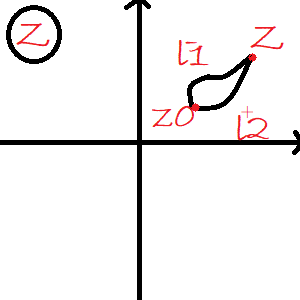
\includegraphics{lec33_2}}
	\[
	l_0 = l_2^+ \cup l_1^+ \implies
	\oint\limits_{l_0} f(t) dt = 0 \implies
	\int\limits_{l_1^+} f(z) dz +
	\oint\limits_{l_2^+} f(z) dz = 0 \implies 
	\int\limits_{l_1^+} f(z) dz =
	\oint\limits_{l_2^-} f(z) dz
	\]
	Также, как и в теореме о существовании ???перв???
	ФКП для \eqref{lec33:13} получаем, что $ \exists \Phi'(z) = f(z) $. 
	Из аналитичности $ \Phi(z) \implies $ 
	аналитичность $ \Phi'(z) \implies $
	аналитичность $ f(z) $ в $ D $.
\end{proof}
\begin{rem}
	По своей сути теоема Мореры является обратной
	к интегральной теорме Коши.
\end{rem}

\end{document}
